\section{\retro System Design}\label{design}
In this section, we describe our design of \retro in more detail. The system consists of a \reader and a \vitag, each of which contains the transmitting and receiving logic. We elaborate their design one by one, starting with the transmitter of the \reader. Its detailed diagram is shown in \figref{fig:diagram_reader}.

%The system consists of \readertx, \readerrx, \tagtx, and \tagrx. The first two belong to the \reader\ and the last two belong to the \vitag.  
\subsection{\readertx Design}
The \readertx employs a standard VLC design as in other work:  it performs encoding using an MCU and toggles the LED light to control the power amplifier. Specifically, we employ a 1MHz carrier and perform on-off keying (OOK) and Manchester coding. The communication bandwidth we use is 10kHz. 

Note that we may use even higher carrier frequency and larger communication bandwidth. We made the choice due to the limitation of ordinary commercial off-the-shelf LED we have. If we toggle at a faster rate, the amplitude difference between On and Off state will be too small to serve as an effective carrier. We use 10kHz bandwidth as it suffices applications we have in mind, e.g., send back the tag ID and certain sensor information it may carry.

%We next focus on the design of the other three components, elaborating on the key design choices. 


\begin{figure}[!th]
\centering
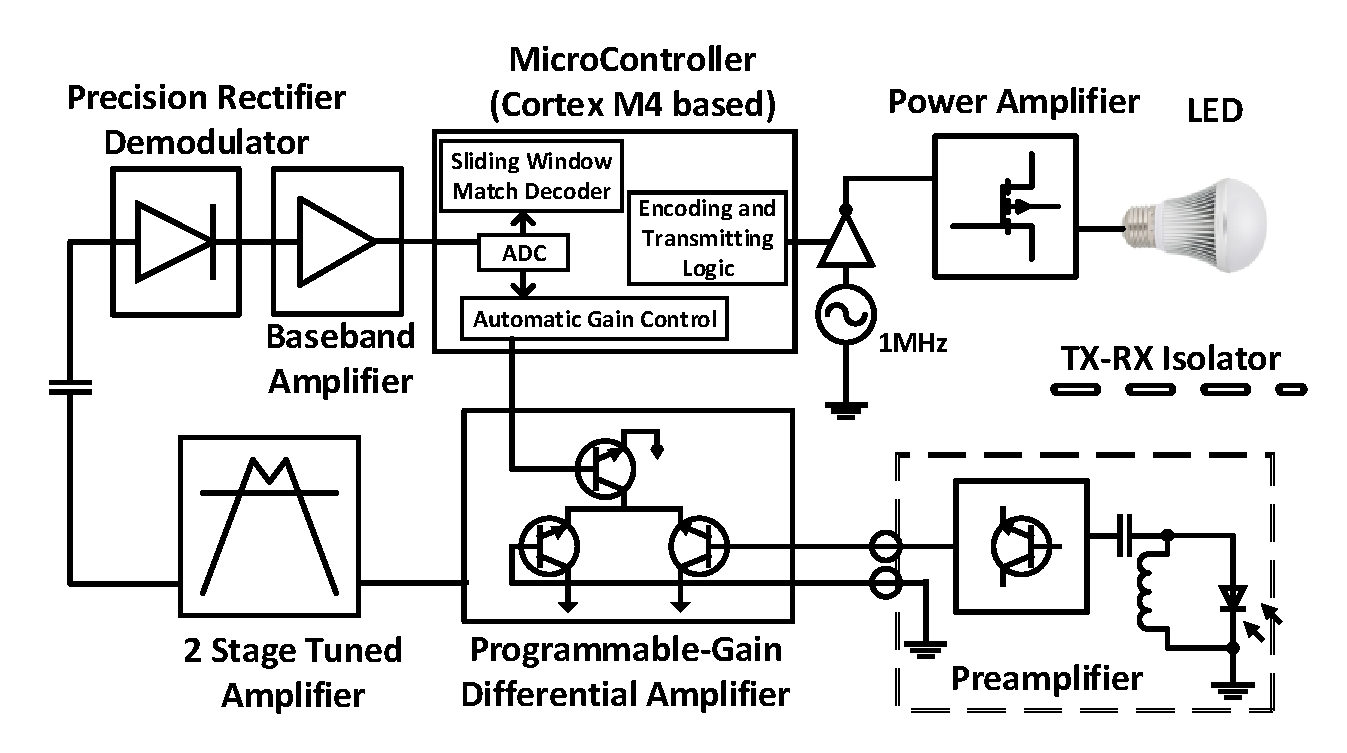
\includegraphics[width=\columnwidth]{fig/read_diagram.pdf}
\vspace{-1em}
\caption{Circuit diagram of \reader. }
\label{fig:diagram_reader}
\end{figure}

\subsection{\readerrx Design}\label{ssec:readerrx}
%\subsection{\reader Transmitter (\readertx)} \label{subsec:LEDtrans}

%As shown in Fig.~\ref{fig:sysdiagram} (b), the transmitter on \reader\ is composed of a crystal oscillator that runs at 1MHz\footnote{The fastest flickering rate of our LED is 1MHz},\remind{Later on when we say using only RC oscillator for energy savings, do we have any measurement of the energy consumption of a crystal oscillator? We need to provide the number. \hl{also the size requirement}} and an MCU followed by two amplifiers. The MCU-generated bits toggle the crystal oscillator to OOK the signal with Manchester encoding. The modulated signal will then be amplified and fed to a LED. To make sure the brightness of the LED does not pose a difference between the transmitting and not transmitting state, we add a DC component to the signal. The magnitude of the DC component is adaptable so that we can dim the brightness of the LED emission. In addition to the dimming support, flickers are avoided in \reader\ transmitter. We use 10kHz as the symbol rate, which far exceeds the frequency (200 Hz) below which human eyes will feel of fluctuations, which could disturbing and unacceptable. 

% We illustrate a typical packet the LED transmits in Fig.~\ref{fig:commdiagram}.

% \begin{figure}[!t]
% \vskip -0.03in
%   \centering
%       {
%         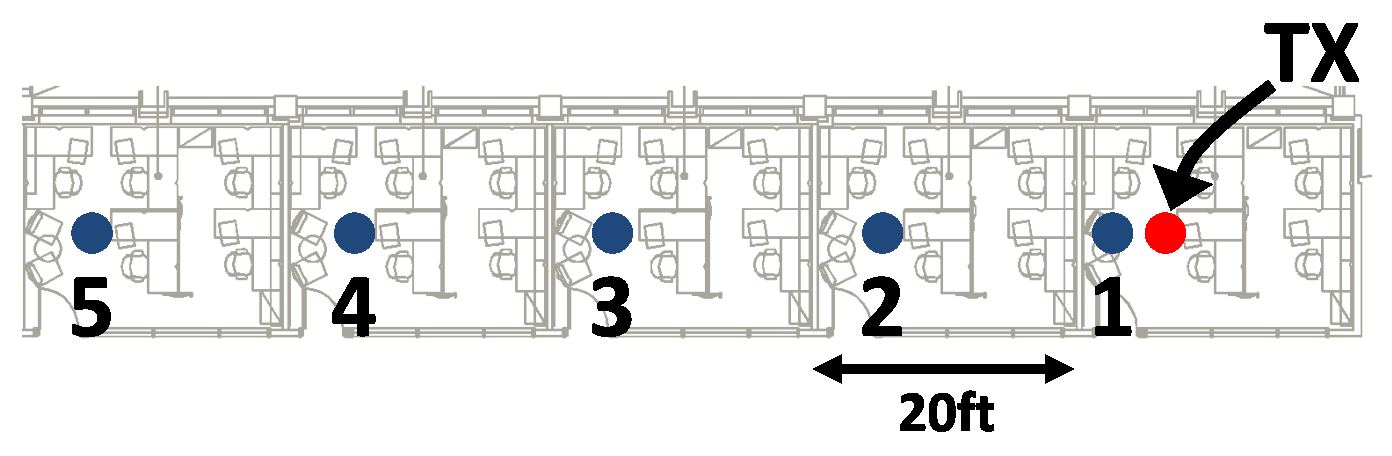
\epsfig{file=../figures/layout2.eps, width=0.6\columnwidth}
%       }
% \caption{{\bf An LED-transmitted Packet} \hl{blah}.}
% \label{fig:commdiagram}
% \vskip -0.05in
% \end{figure}

%\subsubsection{Challenges of \readerrx Design}
%\paragraph{Challenges of \readerrx Design}
The major challenges that arise in the design of the \readerrx are the following. First of all, the signal from the \vitag reflection is extremely weak, especially due to the use of the small retro-reflector on the \vitag. Second, the signal is severely interfered by other light and electrical sources. In particular, as the light sensor sits next to the LED, it is likely that there is leakage from downlink signals and carrier, in additional to the diffusing reflections from the ambient sources. Because of the close distance, the interference is several orders of magnitude greater than the actual reflected signal from the \vitag. As measured \fyi{in one implementation of 12W LED lamp}, the power of the \vitag-reflected signal is about $-80dBm$ \fyi{at 1.5 meters} while the \readertx emitted light signal can be up to $30dBm$. In fact, these interference could cause the \readerrx amplifiers to saturate without careful design. In practice, the light reflected by the movement of humans and other objects around also causes such interference. 
Thirdly, the converted electrical signal is also interfered by commercial FM radios that operate around 1MHz. The harmonics of the $50-60$Hz AC supply of the lighting infrastructure also matters, which is on par with the toggling rate (0.5kHz) of our LCD modulator. %The harmonics be relatively strong than the reflected signal.
%\remind{We may move this AC harmonics to the part explaining the performance differences between indoor and outdoor, as we do not have special treatment of this noise source. or do we???}
Last but not the least, our choice of using a small and low frequency RC oscillator at the \vitag, instead of high-precision oscillator (for sake of energy consumption reduction), makes the reflected signal suffer from clock offsets and drifts.   


In our design, we first try to isolate the receiving path, both the circuit and light sensor, from the transmitting path. In practice, we use 4-layer PCB and always ensure the wires are covered by two copper layers connected to ground. We also shield the light sensor to avoid leakage of the downlink signals. 

In the rest of this section, we elaborate the modular and algorithmic designs of \readerrx that overcome these challenges.  


%\subsubsection{Amplification and Demodulation}
%Since the received signal is extremely weak (the order of uV), we apply four successive RF amplifiers (gain>80dB), an active detector with a high-speed operational amplifier (gain=0dB) and a baseband amplifier (gain=100dB) to achieve superior total performance (gain>100dB). The detailed design is the following. 
\paragraph{Amplification and Demodulation}
As shown in \figref{fig:diagram_reader}, an external light sensor with a parallel inductor captures the \vitag signal and performs preliminary band-pass filtering. The photocurrent is then amplified by a subsequent preamplifier and further transmitted to the internal (\ie on the \reader board hosted within the lamp) amplifier and processing circuit. An impedance matching module is incorporated. 

The pair of transmission lines is relatively long, decoupling the front end and the subsequent processing unit.%and easily interferes with \textit{common-mode noises} such as the radio and AC harmonics. 
As the two wires are equally affected by the common-mode noises, we thus design a tuned differential amplifier as the first-stage internal amplifier. By subtracting the signals from the two wire, the differential amplifier effectively eliminates the common-mode noises. It further suppresses other off-band noises through LC resonance at 1MHz carrier frequency. As the reflected signal from \vitag\ is extremely weak, we further amplify it through two additional LC-structured amplifiers. The overall amplification gain is $80dB$. 
This signal then goes through a high precision envelope detector to pick up the baseband signal from the carrier. 
%, which realizes regular passive diode demodulation that picks out the baseband signal from the $1MHz$ carrier but with much lower distortions. 
Finally, the baseband signal is amplified and fed to the MCU, which performs analog-to-digital conversion and decoding therein. 

Note that the gain of the differential amplifier is programmable and controlled by the micro-controller. We also use two-stage amplifiers (instead of one-stage amplifier with very large gain) both with feedback mechanisms. These mechanisms helps pull the circuit state away from self-excitation. 


%\begin{figure*}[!t]
%\vskip -0.1in
%\centering
%{\footnotesize
%\begin{tabular}{ccccc}
%\epsfig{file=../illustrations/waveform1.eps, width=0.2\columnwidth} & \epsfig{file=../illustrations/waveform2.eps, width=0.2\columnwidth} & \epsfig{file=../illustrations/waveform3.eps, width=0.2\columnwidth} & \epsfig{file=../illustrations/waveform4.eps, width=0.2\columnwidth} & \epsfig{file=../illustrations/waveform5.eps, width=0.2\columnwidth}\\
%{(a) Normal} & {(b) Up-truncated} & {(c) Down-truncated} & {(d) Up and Down-truncated} & {(e) Average-drifted}\\
%\end{tabular}
%}
% \vskip -0.1in
%\vspace{1em}
%\caption{\footnotesize{\bf Varying Wave patterns.} Blah Blah.}
%\label{fig:dynamicRange}
%\vspace{-1em}
%\end{figure*}
%

%\begin{figure*}[!t]
%\centering
%{\small
%\begin{tabular}{cccc}
%\epsfig{file=../illustrations/waveform1.eps, width=0.22\columnwidth} & 
%\epsfig{file=../illustrations/waveform2.eps, width=0.22\columnwidth} & 
%\epsfig{file=../illustrations/waveform3.eps, width=0.22\columnwidth} & 
%\epsfig{file=../illustrations/waveform5.eps, width=0.22\columnwidth}\\
%{(a) Normal} & {(b) Top-truncated} & {(c) Bottom-truncated} & {(d) Average-drifted}\\
%\end{tabular}
%}
% \vskip -0.1in
%\vspace{1em}
%\caption{Possible Waveform patterns after baseband amplifier of \readerrx. \todo{Verify!! Is it from after baseband amp?}}
%\label{fig:dynamicRange}
%\vspace{-1em}
%\end{figure*}


\begin{figure}[!th]
  \begin{center}
      \subfigure[Normal]{
        \includegraphics[width=0.45\columnwidth]{../illustrations/waveform1.eps}\label{fig:waveform1}
      } 
      \hfill
      \subfigure[Top-truncated]{
        \includegraphics[width=0.45\columnwidth]{../illustrations/waveform2.eps}\label{fig:waveform2}
      } \\ \vspace{-1em}
      \subfigure[Bottom-truncated]{
        \includegraphics[width=0.45\columnwidth]{../illustrations/waveform3.eps}\label{fig:waveform3}
      } 
      \hfill
	  \subfigure[Average-drifted]{
        \includegraphics[width=0.45\columnwidth]{../illustrations/waveform5.eps}\label{fig:waveform5}
      } 
\vspace{-1em}
      \caption{Possible waveform patterns after the baseband amplifier of \readerrx. }\label{fig:dynamicRange}
  \end{center}
\vspace{-1em}
\end{figure}

%\subsubsection{Decoding and Handling Clock Drift}\label{subsubsec:clockoffset}
\paragraph{Decoding and Handling Clock Drift}
The clock offset and drift caused by the RC-clock of the \vitag bring challenges as we try to extract the timing information from the signal and perform the decoding at the same time. %First, we describe why common decoding methods do not work in our case.
There are several common decoding methods. One method is based on peak (or edge) detection. Its principle is to extract the extreme (discontinuous) points in the signal to detect clock beats. A second approach is averaging-based algorithm in which signal samples are averaged to generate a threshold, and samples above this threshold denote ones and below denote zeros. A third approach is symbol-based match filter that tries to match the waveform of one symbol and detects the convolution peaks to determine the accurate timing.

\begin{figure}[tb!]
\centering
\includegraphics[width=\columnwidth]{../figures/slidingWindow.eps}
\vskip -0.05in
\caption{All possible 3-bit patterns (left) and illustration of their actual voltage levels (middle), and corresponding matching templates (right) for edge detection. 
}
\label{fig:swmsmf}
\end{figure}


However, none of these methods work for us. 
Take for example the normal signal input waveform shown in \figref{fig:dynamicRange}(a). 
Due to the possible lag of the automatic gain control at the \readerrx, the high dynamic range of interference, we may obtain top- or bottom-truncated waveforms, as shown in \figref{fig:dynamicRange}(b) and (c), or both top- and bottom-truncated waveform (not shown due to space limit). Such situation would fail peak/edge detection algorithms. Similarly, the ambient brightness changes (e.g., caused by human body reflection) will likely cause a time-varying shift in average value, as shown in \figref{fig:dynamicRange}(d). This would fail the averaging-based approach. Furthermore, due to Manchester coding, one bit contains two chips -- a high volt chip followed by a low volt chip, or vice versa, indicating a `0' and `1', respectively. Other than an all `0' or all `1' sequence, the rising edge and the falling edge are not evenly spaced in time. %The correlation peak for such unevenly spaced chips will be skewed. 
%A typical example is three chips that contain one high-volt chip followed by two low-volt chips, in which case the correlation peak will be skewed, compared to the case where the voltage is high for one chip and low for the next. 
This results in two (and at most two) consecutive low (or high) voltage chips for bit sequence `01' (or `10'). 
A low voltage chip corresponds to the LCD discharging phase at the \vitag; Consecutive low chips thus correspond to continuous discharging of the LCD. As a result, the second low chip will have a lower voltage than the first one. Similarly, the second high chip will have a higher voltage than the first one in two consecutive high voltage chips. The consecutive low or high voltage chips and their corresponding voltage level are depicted in \figref{fig:swmsmf}. 
In the face of these distortions, the single-symbol match filter method will fail, because the correlation peak will be skewed for those unevenly spaced high/low voltage chips.

%\vskip 0.05in\noindent{\bf \hl{CDMA-based algorithms}} use a string of chips to represent one bit~\cite{abc1}, and does correlation on the receiver side to decode the bit by finding the peak of the correlation result. The algorithm can pinpoint the clock and hence decode the signal in a low SNR situation, but it is not suitable for low symbol-rate channels like the uplink in our case. 

%\vskip 0.05in\noindent{\bf One-symbol \qm{match filter} algorithms} try to match the wave form of the signal and detects the convolution peaks to determine the accurate timing. However, due to the rough equivalence of the LCD on the tag side that shapes a bit and a capacitor, the basic wave form tends to be sawtooth, as shown in Fig.~\ref{fig:dynamicRange} (a) when there is no top or bottom truncation. Further, as the bits are encoded in Manchester code, the rising edge and the falling edge are not necessarily symmetric in time. A typical example is three chips that contain one high-volt chip followed by two low-volt chips, in which case the correlation peak will be skewed, compared to the case where the voltage is high for one chip and low for the next. Therefore, the timing will be biased.


%\noindent\textbf{\textit{Sliding-window Multi-symbol Match Filter:  }}
We develop a novel algorithm, termed \textit{sliding-window multi-symbol match filter} algorithm, to decode the signals from Manchester coding that subject to a huge dynamic range. %The approach extends the one-symbol match filter to that with an addition regarding clock adjustment using a multi-symbol match filter. 
The basic idea is to avoid the biased timing caused by skewed correlation peaks in the conventional symbol-based match filter method, by matching \textit{all possible patterns} of the waveform that may result from Manchester encoding, and iteratively adjusting the local clock by every bit period. To begin with, the algorithm exploits standard correlation to detect the preamble of a packet. In our design, preambles last for a time period equivalent to 3 Manchester chips.
%\fyi{Preambles are a string of eight `1's in our design. Its chips are evenly distributed and alternating between high and low voltages, and hence can be accurately detected}
%, using the fact that the preamble is different from any possible bit patterns in the payload and is known beforehand. 
Upon finding the preamble, the algorithm estimates the length of a bit using the knowledge of the \vitag clock which is known but subject to offsets and drifting. Then the algorithm iteratively performs the following two steps:
\\[4pt]
\noindent\textit{Step 1: Template Matching.} For all the samples within the three-bit span, we match them against the corresponding template, as shown in \figref{fig:swmsmf}. Note that the template is of amplitude of $\pm1$, so as to most precisely detect the rising or falling edges of the bit in the middle. Ideally, the right correlation yields a peak in the middle of the three bits. 
\\[4pt]
\noindent\textit{Step 2: Local Time Recovery.} 
%Then the algorithm adjusts the clock estimation by correlating the three bits from the raw signal against the corresponding gold pattern from the eight patterns. 
Due to the time variance with the start of the packet and the frequency deviation between the clocks of the \reader and the \vitag, the peak correlation does not necessarily align with the actual timing of the edge. This yields errors in clock estimation. To bound this error as the decoding goes, we perform linear regression $t=k\cdot s+s_0$ to estimate the central time of every three bits, where $s_0$ is the initial time estimate after preamble detection, $s$ and $t$ are the central time from the \reader's view and from the \vitag's view, respectively, and $k$ denotes the clock sampling ratio of the \vitag\ over \reader. Every round $k$ is re-estimated, and then the algorithm moves the three-bit window one bit forward.
 
The whole procedure is repeated till reaching the end of the packet. This time recovery algorithm bounds the error on $t$ from diverging as the decoding process proceeds. %\todo{The proof does bounds $k$. Original text say prevent $k$ from propagating, which is not correct. How about simply put "This time recovery algorithm bounds the estimation error as the decoding proceeds."? Chao: yes, this is more appropriate} 
We formally describe this in the following lemma, for which we give a proof in Appendix.
\begin{lemma}
The time recovery algorithm ensures the error of the \vitag clock estimation to converge to zero asymptotically if a packet contains infinite number of bits. 
\label{lem:lemma1}
\end{lemma}

%Note that we choose a three-bit time span as a correlation unit because three bits are the smallest number of bits that contain all possible wave forms when the signal is Manchester-encoded. The use of three-bit window can maximize the correct detection of the bit in the middle. 


% \begin{figure}[!t]
% \vskip -0.03in
%   \centering
%       {
%         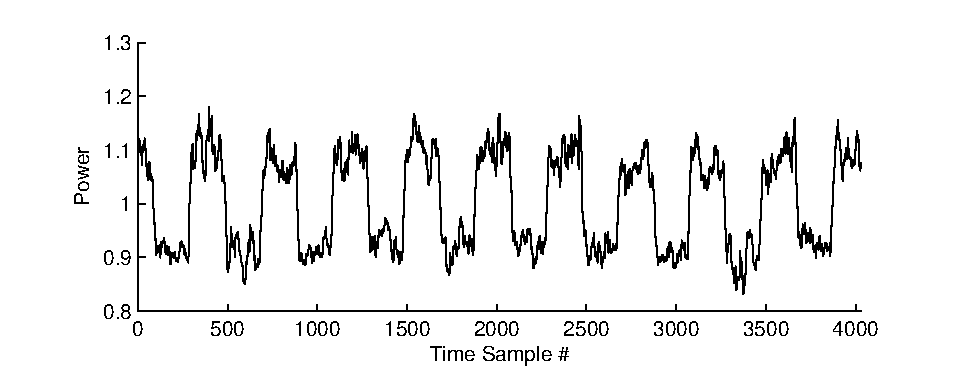
\epsfig{file=../figures/divide.eps, width=0.6\columnwidth}
%       }
% \caption{{\bf Signal Captured by the LED Light Sensor \hl{replace with a system block diagram!!}} \hl{integrates both mmm in a single design. It can operate using both RFID and TV transmissions}.}
% \label{fig:capture}
% \vskip -0.05in
% \end{figure}




%\begin{figure}[!th]
%  \begin{center}
%      \subfigure[Waveform of TP1]{
%        \includegraphics[width=0.4\columnwidth]{../illustrations/waveform_a1.eps}\label{fig:waveformOfTag_Lightsensor}
%      } 
%      \hfill
%%      \subfigure[Waveform of TP2]{
%%        \includegraphics[width=0.45\columnwidth]{../illustrations/waveform_a2.eps}\label{fig:waveformOfTag_Amp}
%%      } \\
%      \subfigure[Waveform of TP3]{
%        \includegraphics[width=0.4\columnwidth]{../illustrations/waveform_a3.eps}\label{fig:waveformOfTag_TunedAmp}
%      } 
%      \\
%	  \subfigure[Waveform of TP4]{
%        \includegraphics[width=0.4\columnwidth]{../illustrations/waveform_a4.eps}\label{fig:waveformOfTag_Dmodulator}
%      } 
%      \hfill    
%	  \subfigure[Waveform of TP5]{
%        \includegraphics[width=0.4\columnwidth]{../illustrations/waveform_a5.png}\label{fig:waveformOfTag_Thresholding}
%      } 
%
%%      \vspace{-1em}
%      \caption{Waveforms at various stages in the \tagrx. \todo{Pay attention to the units/scale. e.g., seems there is no much amplification from (a) to (b).}}\label{fig:waveformOfTag}
%  \end{center}
%%  \vspace{-0.3in}
%\end{figure}
%

\begin{figure}[!th]
\centering
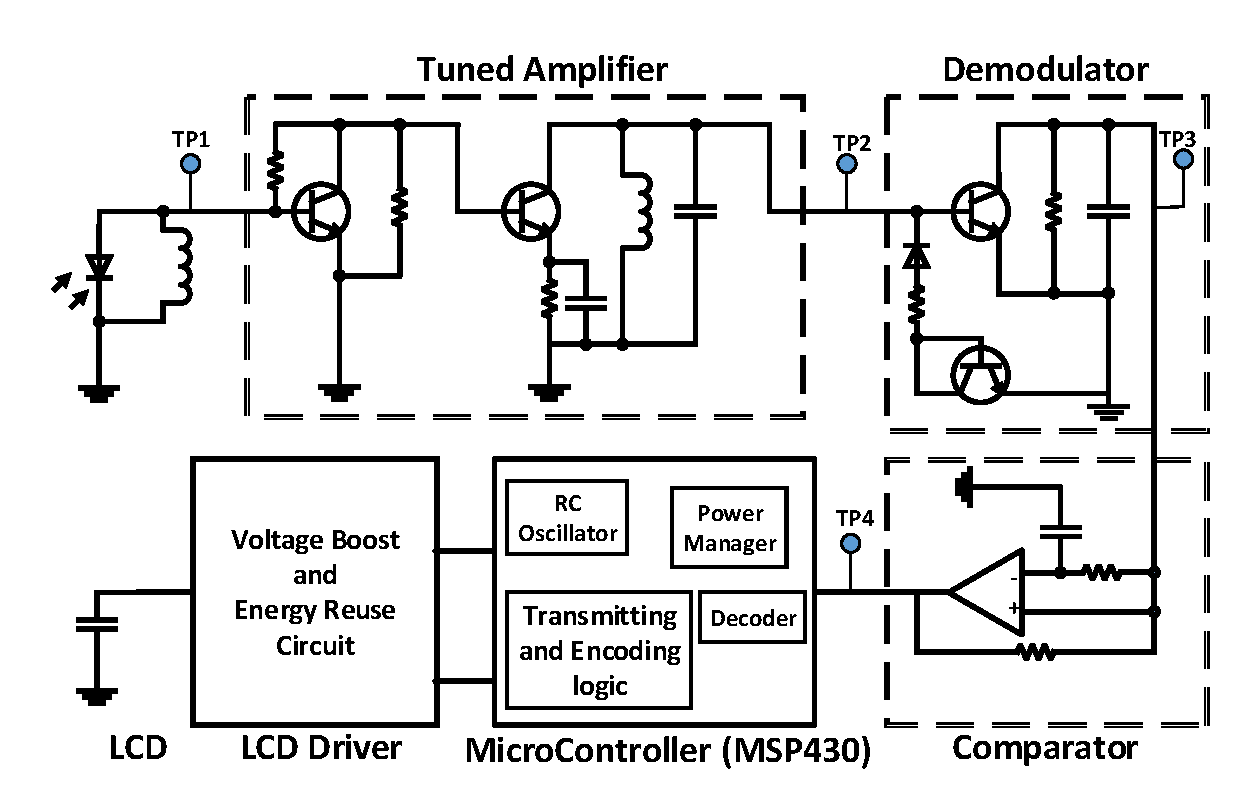
\includegraphics[width=\columnwidth]{fig/tag_diagram.pdf}
\vspace{-1em}
\caption{Circuit diagram of \vitag.}
\label{fig:diagram_tag}
\end{figure}


\subsection{\tagrx Design}

%The major challenge we want to address in the \vitag design is to push to limit the low power consumption. For a normal design, there would be two major energy consumption modules, namely the ADC and digital signal processing (for the \tagrx) and the light emission and modulation (for the \tagtx). The adoption of the retro-reflector removes the energy for emitting light, the modulation (via LCD) still consumes relatively significant energy. In addition, a high accuracy crystal oscillator would incur significant energy overhead. 
For a normal design of \tagrx, the major energy consumption would be from the ADC and digital signal processing. 
In our design, we perform most of the processing in analog domain and avoid using the ADC while retaining accuracy. 

%As shown in \figref{fig:sysdiagram}, the incoming light signal is first captured by the light sensor (photodiode) and converted to electrical signal. The signal is first filtered and then go through tuned amplifiers and a demodulator. It is further amplified and then digitized via a comparator (instead of an ADC).  


%\subsubsection{Demodulation}
\paragraph{Demodulation}
As shown in \figref{fig:diagram_tag}, the incoming light is first captured by the light sensor. 
%As shown in Fig.~\ref{fig:sysdiagram} (b), we use two triode amplifiers combined with a well-designed detector to achieve high gain and extremely low power consumption. \vitag\ captures signals with a light sensor. 
The light sensor has an equivalent capacitance, which, with an inductor parallel to it, makes up a preliminary LC filter. Two triode amplifiers successively amplify the RF signal, after which the signal is passed along for demodulation. 

Our demodulator contains a constant voltage source and a low-pass amplifier. The constant voltage source sets a ultra-low quiescent current that flows into the base of the triode in the low-pass amplifier, making it work at a critical conduction mode, so that the positive half of the signal can pass through and be amplified while the negative part can only make the triode into cut-off mode. Hence, the 1MHz AC carrier is turned into the unipolar signal with a low frequency DC bias which can represent its primary envelope. Finally, the envelope signal is obtained by a smoothing capacitor and then fed into a comparator for digitization. 

%Overall, compared with a commonly used passive diode detector, much higher gain can be provided by our solution which simultaneously consumes quite low energy due to its critical conduction mode.

%\subsubsection{Digitization and Decoding}
\paragraph{Digitization and Decoding}
%While the output of the envelope detector is a smooth wave, it is still analog with continuous values. In principle, a receiver with an ADC can distinguish between the two signal levels by processing the digital samples. Specifically, say we have two signals with different voltages, $V_0$ and $V_1$, $V_0 > V_1$, where $V_0$ and $V_1$ correspond to the power levels for the zero and one bits. To distinguish between them, the receiver would first compute a threshold value. If the duty cycle of the signal is $50\%$, and odds of the occurrence of zeros and ones are equal, then the threshold is the average of the two power levels. If the received signal is greater than this threshold, we conclude that the received signal is $V_1$; else, we conclude that the received signal is $V_0$.
%\fye{To avoid using power-hungry ADCs, we digitize the analog signal with a comparator. Because of the pulse-width modulation (PWM) we adopted, the goal of our design is different from a typical digitization process that involves comparison instant value against the time-average. The PWM-encoded signal uses the width of a pulse to denote bits. Specifically, a wide pulse denotes 1, and a narrow one denotes 0. To align with this pattern, we design the comparator to detect the \textit{change} of the voltage. First, using a resister and a capacitor, the comparator sets a time constant that features its detection delay that corresponds to the input symbol rate. The comparator consistently compares the current (analog) signal voltage $V_{now}$ with that of the last symbol $V_{previous}$. If $V_{now} > V_{previous}$, the comparator outputs `1'; otherwise, it outputs `0'. }%It is easy to see that our design traces the relative changes in the voltage.}
\fyi{To achieve better energy efficiency, power-hungry ADCs should be avoid and MCU should not always be waking-up. We digitize the analog signal with a comparator. For most of the time, the CPU of MCU is sleeping with only one timer running to measure the time. When a positive jump appears on the TP4 shown in \figref{fig:diagram_tag} (i.e., output of the comparator), the CPU of MCU is waken up, and record the time stamp of the timer, then the CPU halt again. Together with the last wake-up time stamp, we can know the period of the clock cycle on the output of comparator. To align with this working pattern, we adopt clock-period coding. For example, a 185us clock period denotes 00, 195us clock cycle denotes 01, 205 us denotes 10, and 215us denotes 11. So we can receive 2 bits with MCU being waken up just one time.}
\fyi{This enables MCU to sleep most of the time, and upon waking up, it records the time stamp, determines the received bits, and goes into sleep mode again. In our implementation, with a MSP430 MCU running at 1MHz, these routines are done within $16us$. So when there is no carrier or no data on the carrier, the MCU sleep for all the time. When the Tag is receiving data, it still sleeps for most of the time, and just work 16us in the receiving cycle of 200us. }
%\todo{I'm not quite sure here. The comparator already outputs 0 or 1, why MCU needs to do it again? Can we annotate $V_{now}$ and $V_{previous}$ in the figure? If you're sure, keep it. } 
%Further, using a traditional passive diode detector would lead to jagged waveform, which would further cause false comparison results at any edge-based comparator. Instead, our comparator design is more suitable for Manchester coding, which is widely adopted for preventing long consecutive $1$s or $0$s in a bit stream, in avoidance of picking a threshold value that would suffer from drifting. 
%\fyi{When a new symbol comes in, MCU is waken up by the comparator output, and then judges the symbol by the continuously working internal timer.}

%\todo{Need serious double check. It seems to me the microcontroller actually performs decoding. If wrong, the highlighted text below needs to be changed accordingly. } %In the receiving phase, microcontroller consumes $120\mu A$.
%Therefore, we are able to use MSP430 working at its lowest frequency as the MCU. 

In summary, we achieve low energy reception at \vitag by using only analog elements and a low-power MCU (MSP430). The MCU is in sleep mode for most of the time. In the analog circuit design, we further set the transistors to work at a lower DC operating point to maximally reduce energy consumption. 




\subsection{\tagtx Design}\label{subsec:tagtrans}

%\begin{tcolorbox}
%\vskip 0.05in\noindent{\bf Challenge:} Transmitting with the LCD at a high toggling frequency consumes even more power than the receiver.
%\vskip 0.05in\noindent{\bf Solution Principle:} Recycle energy spared by the LCD at every toggle; And use an MCU internal RC oscillator instead of the crystal oscillator used in the receiving phase.
%\end{tcolorbox}


Our \vitag\ transmitter transmits by passively backscattering the incoming light. The core of the transmitter is the combination of an LCD and a retro-reflector that serves as a modulator. %To conserve energy, we design an energy reuse module that, in every modulation cycle, recollects $50\%$ of the energy that would have been wasted by the LCD without such a module. 
%To further save energy, instead of using power-demanding crystal oscillators, we use an MCU internal RC oscillator to generate control signals to toggle the LCD. While the RC oscillator does have worse clock stability and a lower frequency, we design modules that address these issues in~\ref{ssec:readerrx}. 
While the LCD has an ultra low quiescent current, more than $70\%$ of the power consumption during transmission is caused by LCD. The reason is that the LCD has a considerable equivalent capacitance ($~9nF$), which must be charged to $5.5V$ to turn the LCD off and be discharged to turn the LCD on. It is this charging-discharging process that consumes energy. To conserve energy, we design an energy reuse module that recycles the discharging current. 
The LCD requires a voltage high enough (\eg at least $5.5V$) to drive it to achieve desired polarization level. This high voltage is nearly 3 times of solar cell's voltage and cannot be directly fed by solar cells. We design a voltage boosting module that achieves this. The overall design of the \vitag transmitter is presented in \figref{fig:diagram_tag}. 

%We now break down the design into the following key points.

%\subsubsection{Modulating the Retro-Reflector with an LCD}
%To avoid actively generating light signals, which may cost way more power than affordable on a battery-free \vitag, we instead take the advantage of retro-reflectors that passively bounce the incoming light back. As described in Section~\ref{sec:background}, the retro-reflector has the merit that it can directionally bounce the light at a direction same as the one the light arrives at. To modulate the light, we cover the retro-reflector with an LCD. As electromagnetic waves hit the LCD, the LCD lets the light pass through or blocks it depending on the polarization, i.e., the orientation of the liquid-crystal molecules, in the LCD, which is controlled by the voltage added on it. If the applied voltage is large enough, the pixels will appear black. 
%The highest voltage applied to our LCD that turns it completely black is $6.1V$, and the lowest voltage with which it starts to be polarized is $2.1V$. We are able to flicker it as fast as $0.5kHz$, making a $200\mu A$ current consumption. Note, that there are other voltage-controlled reflective materials existing that may have higher flicking rate or lower power. Applying one of those in the system might enhance the energy efficiency and the capacity of the system.  

%\subsubsection{Energy Reuse}
\paragraph{Energy Reuse}
%While LCD has a ultra low quiescent current, more than 70\% power consumption of the circuit during the transmitting is caused by LCD. The reason is that LCD has a considerable equivalent capacitance(about 9nF in our case), which must be charged to 5.5V to turn LCD off and be discharged to reopen it. It is the charging-discharging process consumes those energy. Also the voltage, 5.5V, is nearly 3 times of solar cell's voltage, so a low quiescent and high efficiency DC/DC step-up circuit is needed. 
A conventional LCD driving circuit would discharge LCD from the high driving voltage to Ground and thus waste the energy. %If we can recollect this portion of the current during the LCD discharging phase, it will reduce significant power consumption of the whole circuit. In response, 
The design of our energy reuse module is depicted in Fig.~\ref{fig:energyreuse}.  
\begin{figure}[tg]
  \centering
      {
        \epsfig{file=../illustrations/EnergyReuseCircuits_2.eps, width=\columnwidth}
      }
\vspace{-1ex}      
\caption{Energy reuse design for LCD driver. }
\label{fig:energyreuse}
\end{figure}

During the charging phase, the DC/DC boosts voltage supplied by the solar cell to the high voltage needed for driving the LCD towards a blocking state. 
The MCU sets this high voltage on and activates the transistor $Q_0$ (the PNP transistor in the conventional LCD driver module).
%, and at the same time, the MCU sets a low voltage and ensures the NPN transistor $Q_1$ (on the discharging) to a cut-off state. 
This operation puts the LCD into the charging mode and will pump up the voltage of the LCD.
%This voltage, which the MCU sets to open through transistor $Q_0$ (assume $Q_0$ is the name of the PNP transistor in the conventional LCD driver block), applies to the LCD. Because $Q_1$ is set to close, the voltage on the LCD gets to pump up until it reaches the discharging phase.

In the discharging phase, the MCU sets the $Q_0$ to the cut-off state and thus closes the charging path, and activates the NPN transistor $Q_1$ on the discharging path. %Since there is a diode \fyi{(within $Q_1$???)} that \fyi{blocks the only path along which the LCD is supposed to discharge to the ground, the current that flows from the discharging LCD does not go straight to the ground.} 
Unlike a conventional LCD driver that discharges directly to the ground, in our design, the current flows back to the input of DC/DC circuits. This helps reduce the current drawn from the solar cell. Measurements show that the total power consumed by LCD while switching at $0.5kHz$ decreases from $84uA$ to $46uA$ with energy reuse. 

We note two things about our design. First, the two signals controlling the on/off state of LCD are generated by an MCU, and is alternately activated with a short interval ($2us$). This ensures only one transistor of $Q_0$ and $Q_1$ is open at a time and avoids the transient high current that would be caused if both semi-conductive transistors are activated during the switching. Second, the diode $D_0$ is critical. It prevents the charge on the LCD from discharging to the solar cell. Without it, the initial high voltage ($5.5V$) of LCD will be pull down to that of the solar cell ($2.1V$) immediately after $Q_1$ is ON, a high transient current would result and most energy would be wasted on the BE junction of $Q_1$.
%there will be a transient high current that pull the voltage on LCD to the voltage of solar cell immediately after , thus waste most energy on the b-e junction of transistor $Q_1$. 

